\documentclass[11pt, spanish, a4paper, twoside]{article}

% Versión 1.er cuat 2021 Víctor Bettachini < vbettachini@unlam.edu.ar >

\usepackage[T1]{fontenc}
\usepackage[utf8]{inputenc}

\usepackage[spanish, es-tabla]{babel}
% \def\spanishoptions{argentina} % Was macht dass?
% \usepackage{babelbib}
% \selectbiblanguage{spanish}
% \addto\shorthandsspanish{\spanishdeactivate{~<>}}


\usepackage{graphicx}
\graphicspath{{./figuras/}{../LaTeX/}{../figurasLaTeX/}{./figs}}
% \usepackage{float}

\usepackage[arrowdel]{physics}
\newcommand{\pvec}[1]{\vec{#1}\mkern2mu\vphantom{#1}}
% \usepackage{units}
\usepackage[separate-uncertainty= true, multi-part-units= single, range-units= single, range-phrase= {~a~}, locale= FR]{siunitx}
\usepackage{isotope} % $\isotope[A][Z]{X}\to\isotope[A-4][Z-2]{Y}+\isotope[4][2]{\alpha}

\usepackage{tasks}
\usepackage[inline]{enumitem}
% \usepackage{enumerate}

\usepackage{hyperref}

% \usepackage{amsmath}
% \usepackage{amstext}
% \usepackage{amssymb}

\usepackage{tikz}
\usepackage{tikz-3dplot}
\usepackage{tikz-dimline}
\usetikzlibrary{calc}
% \usetikzlibrary{math}
\usetikzlibrary{arrows.meta}
\usetikzlibrary{snakes}
\usetikzlibrary{decorations}
\usetikzlibrary{decorations.pathmorphing}
\usetikzlibrary{patterns}

\usepackage[hmargin=1cm,vmargin=3cm, top= 0.75cm,nohead]{geometry}

\usepackage{lastpage}
\usepackage{fancyhdr}
\pagestyle{fancyplain}
\fancyhf{}
\setlength\headheight{28.7pt} 
\fancyhead[LE, LO]{\textbf{Mecánica Analítica Computacional} }
% \fancyhead[LE, LO]{\textbf{Mecánica General} }
\fancyhead[RE, RO]{\href{https://ingenieria.unlam.edu.ar/}{$\vcenter{\hbox{
\includegraphics[height=1cm]{ambos.pdf}}}$}}
\fancyfoot{\href{https://creativecommons.org/licenses/by-nc-sa/4.0/deed.es_ES}{$\vcenter{\hbox{
\includegraphics[height=0.4cm]{by-nc-sa_80x15.pdf}}}$} \href{https://ingenieria.unlam.edu.ar/}{DIIT - UNLaM}}
\fancyfoot[C]{ {\tiny Actualizado al \today} }
\fancyfoot[RO, LE]{Pág. \thepage/\pageref{LastPage}}
\renewcommand{\headrulewidth}{0pt}
\renewcommand{\footrulewidth}{0pt}

% LTeX: language = es-AR


\begin{document}
\begin{center}
  % \textsc{\large Mecánica general}\\
  \textsc{\large Ligaduras}
\end{center}

\noindent
%De poder resolver estos problemas en forma autónoma puede asumir que adquirió los conocimientos mínimos sobre los temas abordados en la semana.
%No dude en consultar a docentes y compañeros si no puede terminarlos.
Los problemas marcados con (*) tienen alguna dificultad adicional, no dude en consultar.

\begin{enumerate}

\item 
	\begin{minipage}[t][2cm]{0.7\textwidth}
		\textbf{Máquina de Atwood simple}\\
		Obtenga a partir de la ecuación de Euler-Lagrange la aceleración que presentan las pesas de masas \(m_1\) y \(m_2\) que cuelgan de una cuerda de longitud \(\ell\) que pasa por sobre una polea de radio \(R_p\) y masa \(m_p\).
	\end{minipage}
	\begin{minipage}[c][2cm][t]{0.2\textwidth}
		% \hspace{0.5cm}
		\begin{tikzpicture}
	% define constants for tikz
	\def \radius {1.0};
	\def \deltax {1.0};
	\def \boxwidth {\radius/ 2.5};
	\def \boxAheight {-1.5};
	\def \boxBheight {-2.5};
	\def \pende {\radius + \boxwidth + 0.2};
	\def \pendeLeft {-\radius - \boxwidth - 0.2};

	% circle at 0,0
	\draw [thick] (0,0) circle (\radius);
	\filldraw (0,0) circle (1pt);

	% dashed lines from 0.1 at each side of the circle
	\draw [dashed] (0.2,0) -- ({\radius + \deltax},0);
	\draw [dashed] (-0.2,0) -- ({-\radius - \deltax},0);

	% box centred at (-\radius, \boxAheight)
	\draw [thick] (-\radius -\boxwidth, \boxAheight -\boxwidth) rectangle ({-\radius + \boxwidth},\boxAheight + \boxwidth) node [midway] {\(m_1\)}; 
	\draw [thick] ( \radius -\boxwidth, \boxBheight -\boxwidth) rectangle ({ \radius + \boxwidth}, \boxBheight + \boxwidth) node [midway] {\(m_2\)};

	% draw the line connecting the two boxes to the circle
	\draw [very thick] (-\radius, \boxAheight + \boxwidth) -- (-\radius,0);
	\draw [very thick] ( \radius, \boxBheight + \boxwidth) -- (\radius,0); 

	% draw dashed lines for y coordinates from horizontal lines to the height of middle of the boxes
	\draw [-Latex] (\pendeLeft, 0) -- (\pendeLeft, \boxAheight) node [midway, left] {\(y_1\)};
	\draw [-Latex] ( \pende, 0) -- ( \pende, \boxBheight) node [midway, right] {\(y_2\)};

\end{tikzpicture}
		% 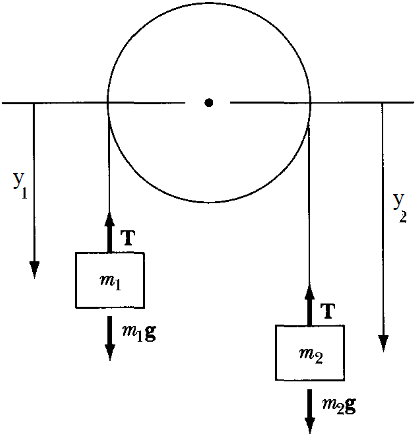
\includegraphics[width=0.75\textwidth]{marion_fig2_11a}
		% 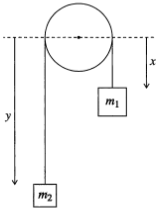
\includegraphics[width=0.75\textwidth]{marion_fig2_1a}
	\end{minipage}
	\begin{enumerate}
		\item Resuelva el caso en que se considera \(m_p\) irrelevante.
		\item Resuelva ahora considerando \(m_p\), y que la polea presenta una sección cilíndrica.
			El momento de inercia de tal cilindro de masa \(m\) ante rotaciones en torno a su eje de simetría longitudinal es \((m/2) R^2\).
	\end{enumerate}


	\item 
	\begin{minipage}[t][1.7cm]{0.75\textwidth}
		\textbf{Péndulo de pesas desilzantes y acopladas}\\ 
		Dos pesas de masa \(m_1\) y \(m_2\) están unidas por una barra rígida inextensible de longitud \(\ell\) y masa despreciable frente a las anteriores.
		La de \(m_1\) puede deslizar sin rozamiento sobre un eje horizontal y la de \(m_2\) en uno vertical.
	\end{minipage}
	\begin{minipage}[c][3cm][t]{0.25\textwidth}
		\begin{tikzpicture}


	% horizontal bar
	\def \barLength {3};
	\def \barAltitude {0};
	\def \barExtra {0.5};
	\draw [thin] (-\barExtra,\barAltitude) -- (\barLength,\barAltitude) node [above left] {\(x\)};

	% vbar
	\def \vbarHorizontal {0};
	\draw [thin] (\vbarHorizontal,\barExtra) -- (\vbarHorizontal, - \barLength) node [above left] {\(y\)};
	
	% weight centres
	\def \hbarWeightAltitude {3* \barLength / 4};
	\coordinate (hbarWeightCentre) at (\hbarWeightAltitude, \barAltitude);
	\coordinate (vbarWeightCentre) at (\vbarHorizontal, - \hbarWeightAltitude);

	% rigid bar joining weights
	\draw [ultra thick] (vbarWeightCentre) -- (hbarWeightCentre) node [midway, right] {\(\ell\)};
	

	% hbar weight
	\def \hbarWeightRadius {.3};
	\shade [ball color=black!80] (hbarWeightCentre) circle (\hbarWeightRadius) node {\color{white} $m_{1}$};

	% vbar weight
	\shade [ball color=black!80] (vbarWeightCentre) circle (\hbarWeightRadius) node {\color{white} $m_{2}$};

	% arc centred at vbarWeightCentre from 45 to 90 with radius hbarWeightRadius + barExtra/2
	\draw [-Latex] (vbarWeightCentre) ++(45:{\hbarWeightRadius + \barExtra}) arc (45:90:{\hbarWeightRadius + \barExtra}) node [midway, above right] {\(\theta\)};
	%\draw [Latex-Latex] (vbarWeightCentre) ++(45:{\hbarWeightRadius + \barExtra}) arc (45:90:{\hbarWeightRadius + \barExtra}) node [midway, above right] {\(\theta\)};

	% \draw [-Latex] (vbarWeightCentre) ++(45:{\hbarWeightRadius + \barExtra / 2}) arc (0:45:{\hbarWeightRadius + \barExtra / 2 }) node [midway, right] {\(\theta\)};
	% \draw [-Latex] (vbarWeightCentre) ++(45:{\hbarWeightRadius + \barExtra / 2}) arc (0:45:{\hbarWeightRadius + \barExtra / 2 }) node [midway, right] {\(\theta\)};


	% horizontal bars joint
	\def \ringRadius {0.1};
	\filldraw (0,0) circle (\ringRadius) node [above left] {\(O\)};
	
	
\end{tikzpicture}
		% \hspace{0.5cm}
		% 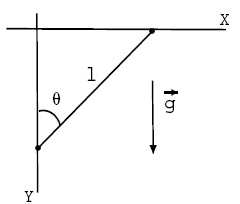
\includegraphics[width=0.75\textwidth]{fcen1-004}
	\end{minipage}
	\begin{enumerate}
		\item Escriba las posiciones de ambas partículas en función de una única coordenada haciendo uso de la ligadura que impone la barra rígida.
		Hágalo para:
		\begin{enumerate*}[
					%itemjoin=\quad,
					%before=\hspace*{\fill},
					%after=\hspace*{\labelwidth}\hspace*{-\labelsep}\hspace*{\fill},
				]
			\item \(y\), la coordenada para la pesa de \(m_2\),
			\item \(\theta\)
		\end{enumerate*} % https://tex.stackexchange.com/questions/591120/how-can-you-put-items-on-one-line-and-center-them
		\item Obtenga las aceleraciones y responda: ¿con cuál coordenada generalizada las expresiones de energía fueron más ``informativas''?\\
		Resultado:
			$\ddot{y} = \frac{- \ell^{2} m_{1} y \dot{y}^{2} + g m_{2} \left(\ell^{2} - y^{2}\right)^{2}}{\ell^{4} m_{2} + \ell^{2} m_{1} y^{2} - 2 \ell^{2} m_{2} y^{2} - m_{1} y^{4} + m_{2} y^{4}}$
			\qquad
			$\ddot{\theta} = \frac{\left(\ell m_{1} \cos{\left(\theta \right)} \dot{\theta}^{2} - \ell m_{2} \cos{\left(\theta \right)} \dot{\theta}^{2} - g m_{2}\right) \sin{\left(\theta \right)}}{\ell \left(m_{1} \cos^{2}{\left(\theta \right)} + m_{2} \sin^{2}{\left(\theta \right)}\right)}$
		\item Realice las sustituciones que corresponden a una aproximación de pequeñas oscilaciones para el caso \(m_1 = m_2 = m\). ¿La expresión de qué sistema obtiene?
		% \item (*) ¿Cuál es el período de movimiento de pequeñas oscilaciones para el caso \(m_1 = m_2 = m\)?
	\end{enumerate}


	\item 
	\begin{minipage}[t][6cm]{0.57\textwidth}
		\textbf{Aro y polea}\\
		Una pesa de masa \(m_{pesa}\) pende de sección de cuerda que sobresale a la derecha de una polea de radio \(R_{polea}\) y masa \(m_{polea}\).
		Tal cuerda, que gira solidaria con la polea, tiene un longitud total \(\ell\) y su masa es despreciable.
		Su otro extremo se ata con un nudo de masa \(m\) a un aro de masa \(m_{aro}\), enrollándose parcialmente en torno a éste.
		El centro de la polea está a una altura \(h_{polea}\) por sobre el del aro de radio \(R_{aro}\) que como puede rotar libremente presenta un momento de inercia \(m_{aro} R_{aro}^2\).
		
		El arco de cuerda enrollada en torno al aro mide un ángulo \(\theta\).
		Tenga en cuenta para escribir la función de ligadura que por el sentido de enrolamiento, al medirse desde la horizontal, tal ángulo presentará valores negativos.
	\end{minipage}
	\begin{minipage}[c][1.5cm][t]{0.2\textwidth}
		\begin{tikzpicture}

	% Ring
	\def \ringRadius {1.0};
	\def \extra {0.8};
	\coordinate (ringCentre) at (0,0);
	\draw [ultra thin] (ringCentre) circle (\ringRadius);	
	\draw [ultra thin] (ringCentre) circle ({\ringRadius - 0.1});	
	\filldraw (ringCentre) circle (1 mm);
	% arc below the Ring
	\def \angle {60};
	\draw [ultra thick] (ringCentre) ++(0:\ringRadius) arc (0:-\angle:\ringRadius);
	% angle dimensions
	\draw [dashed, rotate around={-\angle:(ringCentre)}] {(ringCentre) + (0.2,0)} -- ({\ringRadius + \extra },0);
	\draw [Latex-Latex] (ringCentre) ++(0:{\ringRadius + \extra / 2}) arc (0:-\angle:{\ringRadius + \extra / 2 }) node [midway, right] {\(\theta\)};
	\node [above left] at (\ringRadius/2,0) {\(R_{aro}\)};
	
	% knot
	\shade [ball color=black!80] ($(ringCentre) +({- \angle}:\ringRadius)$) circle(0.25) node [] {\color{white} $m$};

	% draw the pulley
	\def \pulleyRadius {1.5};
	\def \pulleyAltitude {2.5};
	\coordinate (pulleyCentre) at ({\ringRadius + \pulleyRadius}, \pulleyAltitude);
	\fill [inner color = white, outer color = gray!25] (pulleyCentre) circle (\pulleyRadius);	
	\filldraw (pulleyCentre) circle (1 mm);
	
	% rope to ring
	\draw [ultra thick] ($(ringCentre) + (\ringRadius,0)$) -- ($(pulleyCentre) - (\pulleyRadius,0)$) node [above left] {\(\ell\)};
	
	% arc above the pulley
	\draw [ultra thick] (pulleyCentre) ++(0:\pulleyRadius) arc (0:180:\pulleyRadius);
	\node [above] at ($ (pulleyCentre) + (\pulleyRadius/2,0)$) {\(R_{polea}\)};
	
	% height pulley dimension lines
	\draw [dashed] {(ringCentre) + (0.2,0)} -- ({\ringRadius + 2 * \pulleyRadius + 2* \extra},0);
	% \draw [dashed] {(pulleyCentre) + (0.2,0)} -- ($ (pulleyCentre) + (\pulleyRadius,0)$) ;
	\draw [dashed] {(pulleyCentre) + (0.2,0)} -- ($ (pulleyCentre) + (\pulleyRadius + 2 * \extra,0)$) ;
	\draw [Latex-Latex] ($ (pulleyCentre) + (\pulleyRadius + 1.5 * \extra,0)$) -- ($ (pulleyCentre) + (\pulleyRadius + 1.5 * \extra, {- \pulleyAltitude})$) node [midway, right] {\(h_{polea}\)};
	
	% ceiling
	\def \ceilingAbove {2.0};
	\draw [line width = 1 mm] ($(pulleyCentre) + (0,\ceilingAbove)$) -- (pulleyCentre);
	\draw [ultra thick] ($(pulleyCentre) + ({- \pulleyRadius},\ceilingAbove)$)  -- ($(pulleyCentre) + (\pulleyRadius,\ceilingAbove)$);
	\fill [pattern = north east lines] ($(pulleyCentre) + ({- \pulleyRadius},\ceilingAbove)$)  rectangle ($(pulleyCentre) + (\pulleyRadius, {\ceilingAbove + 0.2 })$);

	% weight at rope's end
	\def \weightAltitude {-1.5};
	\def \weightHeight {.5};
	\def \weightWidth {0.5};
	\coordinate (weightCentre) at ({\ringRadius + 2* \pulleyRadius}, \weightAltitude);
	
	% rope to weight
	\draw [ultra thick] ({\ringRadius + 2* \pulleyRadius}, \pulleyAltitude) --(weightCentre);
	
	% weight dimension lines
	\draw [dashed] (weightCentre) -- ({\ringRadius + 2 * \pulleyRadius + 2* \extra}, \weightAltitude);
	\draw [Latex-Latex] ($ (pulleyCentre) + (\pulleyRadius + 1.5 * \extra, {- \pulleyAltitude})$) --  ($ (pulleyCentre) + (\pulleyRadius + 1.5 * \extra, {- \pulleyAltitude + \weightAltitude})$) node [midway, right] {\(y_{pesa}\)};

	% weight 
	\shade [ball color=black!80] (weightCentre) circle (\weightHeight) node {\color{white} $m_{pesa}$};


	% floor
	\def \floorAltitude {-2.0};
	\draw [ultra thick] (-\ringRadius,\floorAltitude) -- (\ringRadius,\floorAltitude);
	\fill [pattern = north east lines] (- \ringRadius,{\floorAltitude-0.2}) rectangle (\ringRadius,\floorAltitude);
	% base of the ring
	\draw [line width = 1 mm] (0,\floorAltitude) -- (ringCentre);


\end{tikzpicture}
	\end{minipage}
	%\begin{minipage}[c][0cm][t]{0.2\textwidth}
		%\hspace{0.5cm}
		%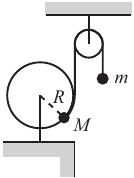
\includegraphics[width=0.75\textwidth]{cmchap6_fig6_14}
	%\end{minipage}
	\begin{enumerate}
		\item Escriba la posición de las partículas con masa en función de \(y_{pesa}\), \(\ell\) y \(\theta\) en un sistema de referncia con origen en el centro del aro.
		\item Describa la función de ligadura y utilícela para expresar las posiciones en función de \(\theta\).
		Verifique su solución revisando que una variación de \(\theta\) ``hacia su cero'' implique que la pesa ``baja''. 
		\item Obtenga la ecuación de Euler-Lagrange para la dinámica sin olvidar los momentos involucrados.\\
		Resultado:
		\(
		R_{aro}^{2} m \ddot{\theta} + R_{aro}^{2} m_{aro} \ddot{\theta} + R_{aro} g m \cos{\left(\theta \right)} + R_{polea}^{2} m_{pesa} \ddot{\theta} + \frac{R_{polea}^{2} m_{polea} \ddot{\theta}}{2} - R_{polea} g m_{pesa} = 0
		\)
	\end{enumerate}


	\item
	\begin{minipage}[t][10cm]{0.65\textwidth}
		\textbf{Maquina de Atwood compuesta} [Marion (english) ex. 7.8]\\ 
		\begin{enumerate}
			\item Escriba la posición de las tres pesas y de la polea inferior en función de 
			las cuatro coordenadas generalizadas indicadas en la figura: \(y_i\) con \(i = 1,2,3,p\). 
			\item Modele las ligaduras que proveen las cuerdas en dos funciones.
			\item Haciendo uso de estas últimas reemplace en las posiciones para expresarles en función de solo dos \(y_i\).
			\item Calcule energías potenciales y cinéticas contemplando los momentos de inercia de las poleas.
			Recuerde la relacíón entre el perímetro (circunferencia) de un círculo y su radio para escribir la velocidad angular en función del \(\dot{y}_i\) correspondiente.
			\item Obtenga las dos ecuaciones de Euler-Lagrange.\\
			Resultados:\\
			% reduce size of equations
			\scalebox{0.9}{
			$- g m_{1} + g m_{2} + g m_{3} + g m_{p} + m_{1} \ddot{y}_{1} + m_{2} \ddot{y}_{1} - m_{2} \ddot{y}_{2} + m_{3} \ddot{y}_{1} + m_{3} \ddot{y}_{2} + \frac{3 m_{p} \ddot{y}_{1}}{2} = 0$}\\
			\scalebox{0.9}{
			$- g m_{2} + g m_{3} - m_{2} \ddot{y}_{1} + m_{2} \ddot{y}_{2} + m_{3} \ddot{y}_{1} + m_{3} \ddot{y}_{2} + \frac{m_{p} \ddot{y}_{2}}{2} = 0$
			}
			\item Resuelva este sistema de ecuaciones para obtener las dos correspondientes aceleraciones generalizadas y con estas escribir las aceleraciones de los cuatro cuerpos en cuestión.\\
			Resultados:\\
			$\ddot{y}_{1} = \frac{4 g m_{1} m_{2} + 4 g m_{1} m_{3} + 2 g m_{1} m_{p} - 16 g m_{2} m_{3} - 6 g m_{2} m_{p} - 6 g m_{3} m_{p} - 2 g m_{p}^{2}}{4 m_{1} m_{2} + 4 m_{1} m_{3} + 2 m_{1} m_{p} + 16 m_{2} m_{3} + 8 m_{2} m_{p} + 8 m_{3} m_{p} + 3 m_{p}^{2}}$\\
			$\ddot{y}_{2} = \frac{8 g m_{1} m_{2} - 8 g m_{1} m_{3} + 2 g m_{2} m_{p} - 2 g m_{3} m_{p}}{4 m_{1} m_{2} + 4 m_{1} m_{3} + 2 m_{1} m_{p} + 16 m_{2} m_{3} + 8 m_{2} m_{p} + 8 m_{3} m_{p} + 3 m_{p}^{2}}$\\
			% $\ddot{y}_{3} = - \frac{8 g m_{1} m_{2} - 8 g m_{1} m_{3} + 2 g m_{2} m_{p} - 2 g m_{3} m_{p}}{4 m_{1} m_{2} + 4 m_{1} m_{3} + 2 m_{1} m_{p} + 16 m_{2} m_{3} + 8 m_{2} m_{p} + 8 m_{3} m_{p} + 3 m_{p}^{2}}$\\
			% $\ddot{y}_{p} = - \frac{4 g m_{1} m_{2} + 4 g m_{1} m_{3} + 2 g m_{1} m_{p} - 16 g m_{2} m_{3} - 6 g m_{2} m_{p} - 6 g m_{3} m_{p} - 2 g m_{p}^{2}}{4 m_{1} m_{2} + 4 m_{1} m_{3} + 2 m_{1} m_{p} + 16 m_{2} m_{3} + 8 m_{2} m_{p} + 8 m_{3} m_{p} + 3 m_{p}^{2}}$
		\end{enumerate}
	\end{minipage}
	\begin{minipage}[c][0cm][t]{0.3\textwidth}
	%		\begin{tikzpicture}
	%			\draw [ultra thick] (-2,4) -- (2,4);
	%			\fill [pattern = north east lines] (-2,4) rectangle (2,4.2); % techo
	%			\draw (0,4) -- (0,3); % linea vertical techo - polea superior
	%			\draw (0,3) circle [radius=0.5]; % polea superior
	%			\draw (-0.5,3) -- (-0.5,1.5); % linea vertical izquierda polea sup - inf
	%			\draw (0.5,3) -- (0.5,2.25); % linea vertical izquierda polea sup - m3
	%			\draw (0.25,1.75) rectangle (0.75,2.25) node [anchor= north west] {\(m_3\)} ; % m3
	%			% \draw (0.25,1.75) node [above=1, right=9.6] {\(m_3\)} rectangle (0.75,2.25) node [above=1, right=9.6] {\(m_3\)} ; % m3
	%			\draw (-0.5,1.5) circle [radius=0.5]; % polea inferior
	%			\draw (-1,1.5) -- (-1,.25); % linea vertical izquierda polea inf - m1
	%			\draw (-1.25,-.25) rectangle (-0.75,0.25) node [anchor= north west] {\(m_1\)} ; % m1
	%			\draw (0,1.5) -- (0,1); % linea vertical izquierda polea inf - m2
	%			\draw (-.25,.5) rectangle (.25,1) node [anchor= north west] {\(m_2\)} ; % m2
	%		\end{tikzpicture}
		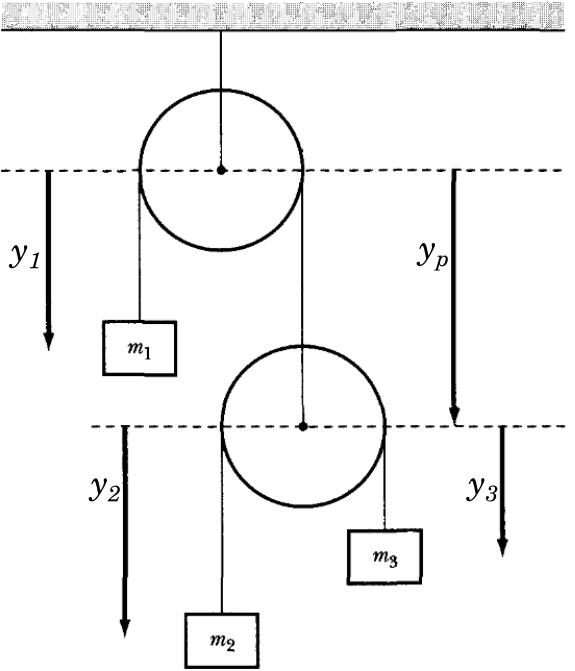
\includegraphics[width=\textwidth]{marion_fig7_6}
	\end{minipage}



\end{enumerate}
\end{document}
